\documentclass{article}

\usepackage{graphicx}
\usepackage{tikz}
\usepackage{tikzsymbols}
\usetikzlibrary{calc,patterns,shapes.geometric}
\pagestyle{empty}
\usepackage[margin=0pt]{geometry}
\geometry{papersize={14in,12in}}

\def\centerarc[#1](#2)(#3:#4:#5){\draw[#1] ($(#2)+({#5*cos(#3)},{#5*sin(#3)})$) arc (#3:#4:#5);}

\begin{document}
	\begin{figure}
		\centering
		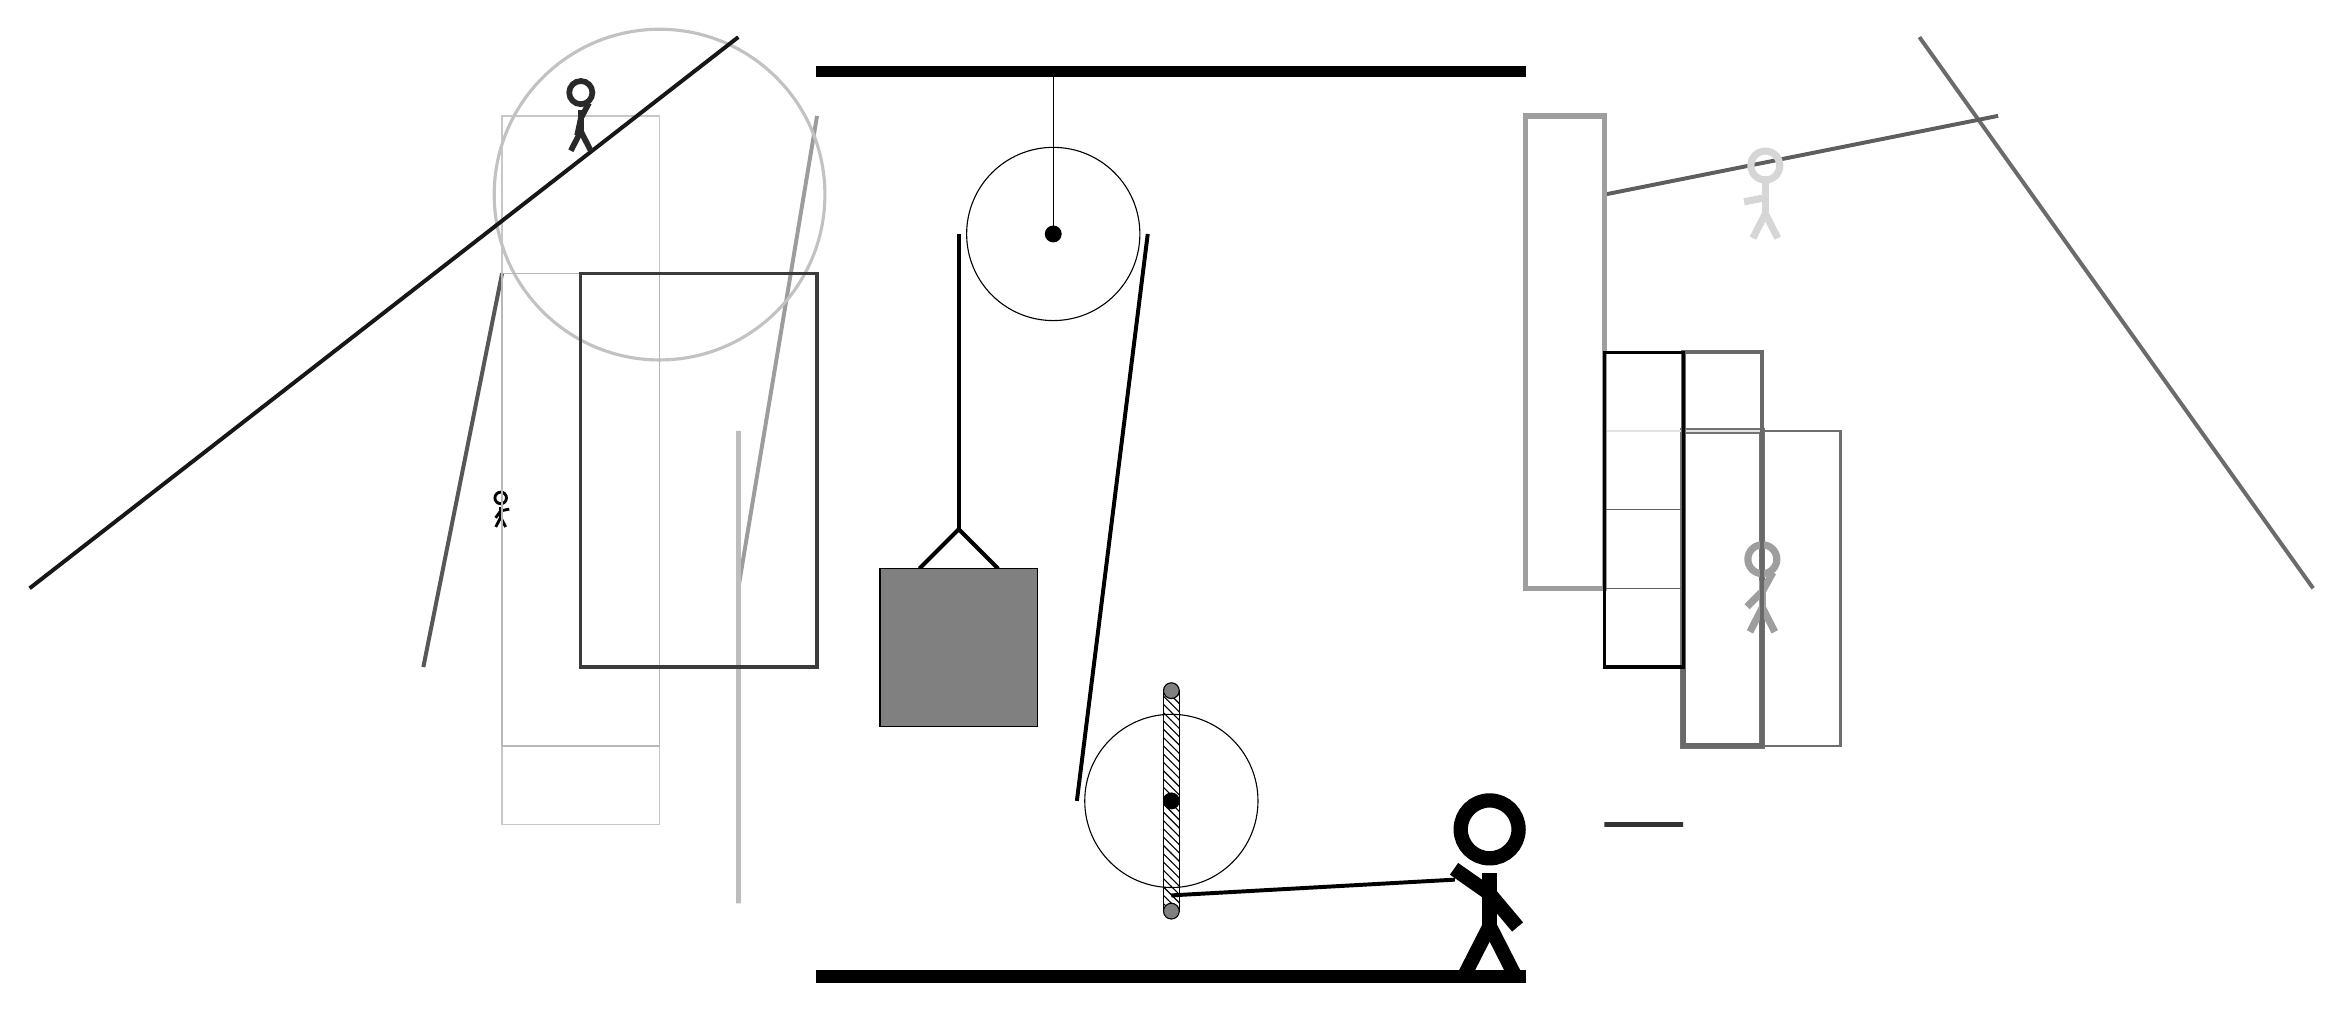
\begin{tikzpicture}
			%%%%% START %%%%%
			
			\draw[fill=black] (-2, 11.5) rectangle (7, 11.625);
			
			\draw (1, 9.5) circle (1.1);
			\draw[fill=black] (1, 9.5) circle (0.1);
			\draw (1, 11.5) -- (1, 9.5);
			
			\draw[fill=white](2.5, 2.3) circle (1.1);
			\draw[fill=black] (2.5, 2.3) circle (0.1);
			\draw[pattern=north west lines, pattern color=black] (2.4, 3.7) rectangle (2.6, 0.9);
			\draw[fill=black!50] (2.5, 3.7) circle (0.1);
			\draw[fill=black!50] (2.5, 0.9) circle (0.1);
			
			\draw[line width=0.5mm] (-0.7, 5.25) -- (-0.2, 5.75) -- (0.3, 5.25);
			\draw[fill=black!50] (-1.2, 5.25) rectangle (0.8, 3.25);
			
			\draw[line width=0.5mm] (-0.2, 9.5) -- (-0.2, 5.75);
			\centerarc[line width=0.5mm](1, 9.5)(0:180:1.2000000000000002);
			\draw[line width=0.5mm](2.2, 9.5) -- (1.3, 2.3);
			\centerarc[line width=0.5mm](2.5, 2.3)(180:270:1.2000000000000002);
			\draw[line width=0.5mm](2.5, 1.1) -- (6.1, 1.3);
			
			\node[line width=0.4mm, color=black!99] at (-6, 6) {\Strichmaxerl[2][54][11]};
			
			\draw [line width=0.6mm, color=black!93](-6, 10) circle (0.0);
			\draw[line width=0.5mm, color=black!39](-3, 5) -- (-2, 11);
			\draw[line width=0.5mm, color=black!58](12, 12) -- (17, 5);
			\draw[line width=0.7mm, color=black!55] (9, 7) rectangle (10, 3);
			\node[line width=0.5mm, color=black!38] at (10, 5) {\Strichmaxerl[5][45][61]};
			
			\draw[line width=0.2mm, color=black!22] (-4, 2) rectangle (-6, 11);
			\draw[line width=0.5mm, color=black!63](8, 10) -- (13, 11);
			\node[line width=0.7mm, color=black!16] at (10, 10) {\Strichmaxerl[5][11][90]};
			
			\draw[line width=0.3mm, color=black!57] (9, 7) rectangle (11, 3);
			\draw[line width=0.2mm, color=black!61] (9, 10) rectangle (9, 10);
			\draw[line width=0.3mm, color=black!12] (-3, 3) rectangle (-3, 2);
			\draw [line width=0.4mm, color=black!24](-4, 10) circle (2.1);
			
			\draw[line width=0.5mm, color=black!91](-3, 12) -- (-12, 5);
			\draw[line width=0.5mm, color=black!66](-6, 9) -- (-7, 4);
			\draw[line width=0.2mm, color=black!11] (8, 7) rectangle (10, 7);
			
			\draw[line width=0.6mm, color=black!59] (9, 8) rectangle (10, 3);
			\node[line width=0.3mm, color=black!84] at (-5, 11) {\Strichmaxerl[4][78][62]};
			\draw[line width=0.7mm, color=black!38] (8, 11) rectangle (7, 5);
			
			\draw[line width=0.7mm, color=black!80] (9, 2) rectangle (8, 2);
			\draw[line width=0.2mm, color=black!61] (8, 5) rectangle (9, 6);
			
			\draw[line width=0.6mm, color=black!26] (-3, 1) rectangle (-3, 7);
			\draw[line width=0.4mm, color=black!99] (8, 4) rectangle (9, 8);
			\draw[line width=0.2mm, color=black!28] (-4, 3) rectangle (-6, 9);
			\draw[line width=0.4mm, color=black!77] (-2, 4) rectangle (-5, 9);
			
			\node at (6.5, 1.2) {\Strichmaxerl[10][-35][-50]};
			
			\draw[fill=black] (-2, 0) rectangle (7, 0.15);
			
			%%%%% END %%%%%
		\end{tikzpicture}
	\end{figure}	
\end{document}